\chapter{Análisis de Impacto}
\label{cap:ImpactoMedioAmbiente}

En 2015, la ONU aprobó la \emph{Agenda 2030 sobre el Desarrollo Sostenible}\cite{agenda2030}, una oportunidad para que los países y sus sociedades evolucionen y mejoren la vida de todos, sin dejar a nadie atrás. Constituye un llamamiento universal a la acción para poner fin a la pobreza, proteger el planeta y mejorar la vida de personas y animales. Se aprobaron entonces 17 objetivos\cite{17objetivos} a alcanzar en 15 años. \\

Dentro de los 17 objetivos, hay 2 muy importantes en los que la aplicación Estublock juega un papel. La tecnología blockchain aporta sin duda una gran cantidad de ventajas, como la fiabilidad, transparencia de las operaciones (el código de los smart contracts esta a disposición de la gente), seguridad de los datos, inmutabilidad, anonimato\dots Pero, estas ventajas traen consigo una pequeña desventaja a nivel medioambiental. Como sabemos, una red blockchain es \emph{descentralizada}, esto se debe a que hay varios nodos conectados entre si. Cada nodo es un ordenador en constante ejecución lo que repercute en el consumo de electricidad. Esto multiplicado por cada ordenador que hay en la red blockchain. Por ejemplo, la red de bitcoin dispone a día de hoy \textit{2021-05-24} de 9786 nodos\cite{bitcoinNodos} lo cuales consumen bastante energía\ref{fig:electricidad_bitcoin}. \\

\begin{figure}[h!]
  \centering
  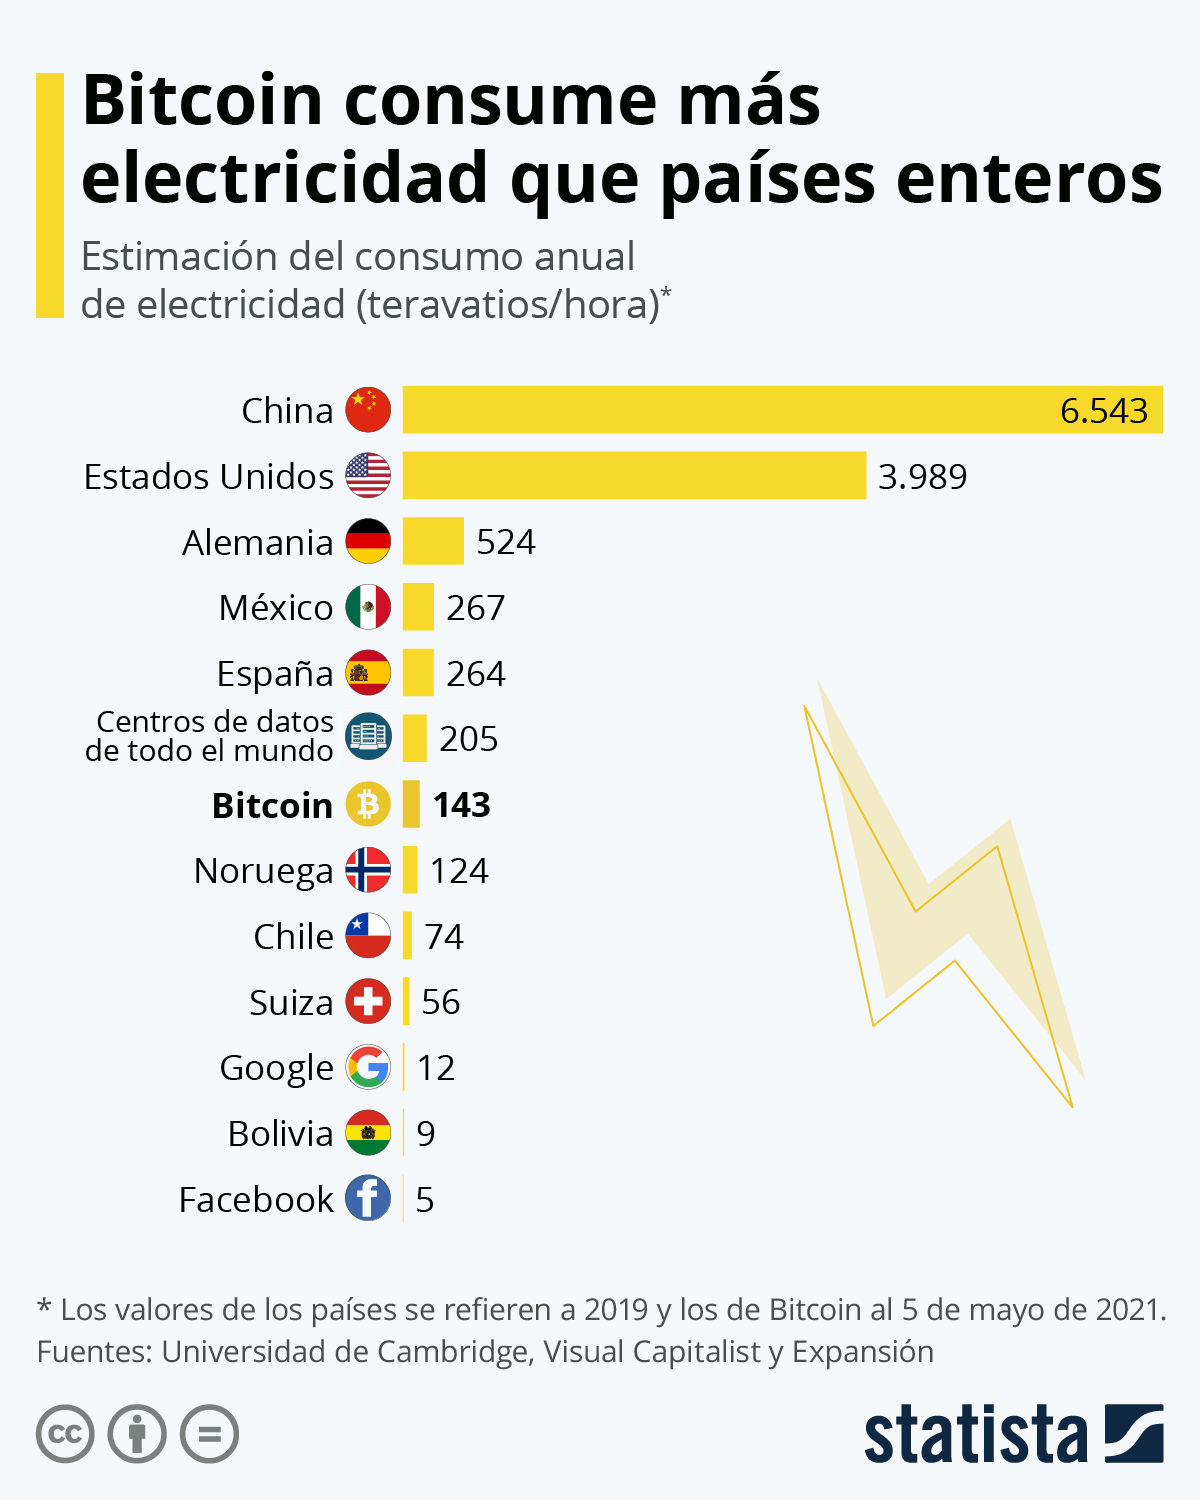
\includegraphics[width=0.8\linewidth]{figs/ImpactoMedioAmbiente/electricidad_bitcoin}
  \caption[Consumo eléctrico de bitcoin]{Consumo eléctrico de bitcoin (\href{https://es.statista.com/grafico/18630/consumo-de-electricidad-anual-de-bitcoin/}{Statista})}
  \label{fig:electricidad_bitcoin}
\end{figure}

Por suerte, aunque parezca que blockchain va a consumir tanta energía como el \textit{Centro de Datos de Todo el Mundo}, en 2019 \emph{Coinshares} realizó una investigación\cite{coinshare} que reveló que el 74\% de las operaciones mineras se realizan con energía renovable, por lo que el impacto medioambiental es menos grave de lo que podría ser. Sin embargo, siempre se puede mejorar, y llegar al 100\% de consumo con energías renovables. \emph{Ethereum versión 2}\cite{Ethereum2.0} es la alternativa verde a este problema, al cambiar el algoritmo de consenso de \textit{Proof of Work} a \textit{Proof of Stake}, ethereum disminuirá casi completamente el consumo de energía. Hasta tal punto, de que \textbf{Joseph Pallant}, fundador de la \emph{blockchain for climate foundation}\cite{bkClimateF} (una fundación que busca utilizar la tecnología blockchain para lidiar con problemas relaciodos con el cambio climático) utiliza Ethereum2.0. Aunque esta segunda versión de Ethereum ya esta en funcionamiento, se requiere de un tiempo para migrar los datos de la versión 1 a la 2, pero con el tiempo la versión 2 de ethereum crecerá, disminuyendo enormemente el gasto energético que conlleva. \\

Aunque Estublock utiliza actualmente la red de Ethereum1.0, su gasto energético es de todos modos casi nulo (pues no hay suficiente tráfico como para que suponga un gasto energético grande), pero hay que tener en cuenta que aunque la red gaste poco, hay varios ordenadores encendidos consumiendo energía, por lo que habrá que migrar a Ethereum2.0 cuando sea posible. Aunque el gasto energético es muy bajo, no se debe olvidar que gastar energía, gasta y que sería recomendable lograr que los ordenadores estén lo más especializados posible para minimizar al máximo el gasto energético cumpliendo con el objetivo \textit{9.4} ``modernizar la infraestructura para que sean sostenibles''. ``Estublock'' tiene también un impacto en el punto \textbf{13} ``Acción por el Clima'' con respecto al objetivo de minimizar las emisiones de carbono al máximo, en las universidades en las que se utilice la aplicación ``Estublock'' y dispongan de nodos en la red blockchain, se puede tratar de utilizar siempre energías renovables como poner paneles solares en la universidad para que los nodos de la red utilicen esa energía renovable para funcionar.

